\begin{surferPage}[Barth'ın Altıgili]{Barth'ın Altıgili}
Derecesi  $6$ olan bu yüzey (altıgil) Wolf Barth tarafından 1996'da inşa edildi.
    
Barth'ın Altıgilinin toplam $65$ tekilliği var.
%    (wenn man die $15$ im Bild nicht sichtbaren, ``unendlich fernen'', mitzählt)%
Bu inşadan hemen sonra Jaffe ve Ruberman, bu sayının bir altıgilin sahip olabileceği en fazla tekillik sayısı olduğunu gösterdi --- dolayısıyla  Barth'ın dünya rekorunu kimse geçemezdi!


Barth'ın inşası büyük sürpriz oldu çünkü uzun zamandır derecesi $6$ olan yüzeylerin yalnızca $64$ tekilliğe sahip olabileceği düşünülüyordu.

İnşanın çarpıcı bir özelliği yirmiyüzlü simetrisine sahip olması; aşağıdaki şekil bir yirmiyüzlü ve simeri düzlemlerini gösteriyor:
%    Die Abb.\ zeigt diesen platonischen Körper und seine Symmetrie - Ebenen: 
%    und diese Ebenen gemeinsam mit der Barth Sextik in einem Bild.     
    % 
  \begin{center}
      \vspace*{-0.1cm}
      \begin{tabular}{@{}c@{\ \ }c@{\,}c@{}}
        \begin{tabular}{@{}c}
          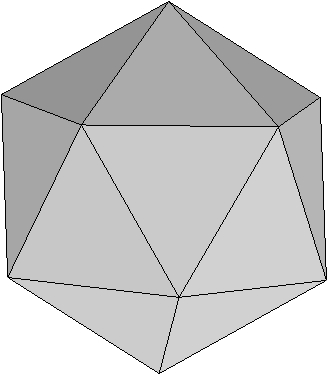
\includegraphics[width=1.4cm]{./../../common/images/icosah}
        \end{tabular}
        &
        \begin{tabular}{@{}c}
          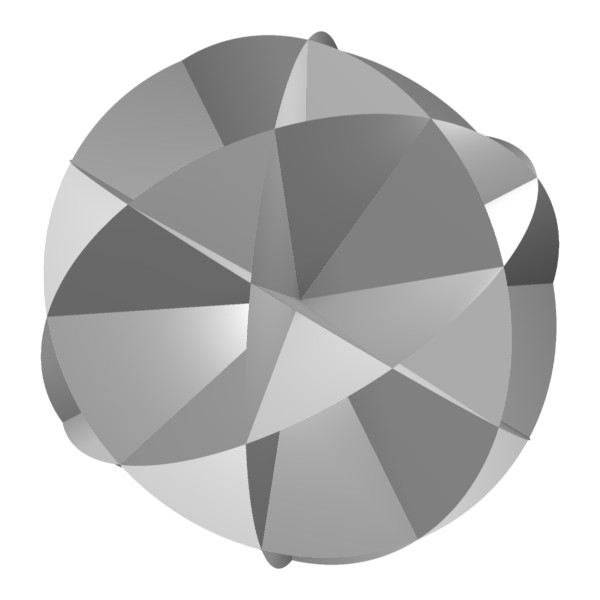
\includegraphics[width=1.4cm]{./../../common/images/barth_sextic_planes}
        \end{tabular}
        &
        \begin{tabular}{c@{}}
          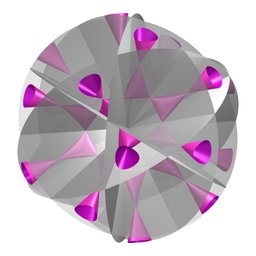
\includegraphics[width=1.4cm]{./../../common/images/barth_sextic_and_planes}
        \end{tabular}
      \end{tabular}
    \end{center}
    \vspace*{-0.1cm}

    Barth'ın Altıgili 
    $P_6 - \alpha K^2=0,$ denklemini sağlar;  burada $P_6$ altı adet simetri düzleminin polinomlarının çarpımı,  $K=x^2+y^2+z^2-1$ birim küre (1 yarıçaplı ve merkezi orijin olan küre) ve 
    $\alpha=\frac{1}{4}(2+\sqrt{5})$.
\end{surferPage}
